\documentclass[11pt,letterpaper]{article}

\usepackage[margin=0.85in]{geometry}
\usepackage{booktabs}
\usepackage{longtable}
\usepackage{tabularx}
\usepackage{array}
\usepackage{pdflscape}
\usepackage{xcolor}
\usepackage{hyperref}
\usepackage{enumitem}
\usepackage{graphicx}

\hypersetup{colorlinks=true, linkcolor=blue!60!black, urlcolor=blue!60!black}
\setlist[itemize]{leftmargin=1.2em,itemsep=2pt,topsep=3pt}
\setlength{\parskip}{5pt}
\setlength{\parindent}{0pt}

\graphicspath{{scoring/report_figs/}}

\newcommand{\code}[1]{\texttt{#1}}
\newcommand{\est}{\emph{estimate}}
\newcommand{\obs}{\emph{observed}}

\title{\textbf{Replication Resource Assessment, Per-Stage Analysis, and Scaling Projections}\\
\large REPLICATE Project --- v2 (44 papers, multi-stage)}
\author{Rick Stevens \and Ollie (OpenClaw subagent ensemble)\\Argonne National Laboratory}
\date{April 25, 2026}

\begin{document}
\maketitle

\begin{abstract}
We report on the agent-driven replication of 44 computational papers spanning mathematics, machine learning, physics simulation, computational chemistry, materials, bioinformatics, electromagnetics, combustion, astrophysics, and PDE numerical methods. Across all 44 replications, mean coverage was 6.70/10 and mean agreement 7.16/10, with a total observed compute footprint of approximately 412 GPU-hours and 144 CPU-hours, 40.7\,M tokens, and 261 wall-hours of subagent runtime, at an aggregate cost of approximately \$1644 (median \$20/paper). The portfolio was assembled in six stages: an initial 30-paper parallel batch, two PDE corpus-mining waves of 5 papers each, targeted retries that doubled the agreement score on weak entries, and an HPC ensemble of the most compute-heavy paper across uicgpu/Polaris/Aurora/chiatta00. We project that, at current per-paper cost and quality, replicating the entire annual computational+theory output of the U.S.\ DOE Office of Science (\textasciitilde{}3,500 papers/yr) costs \$131K /yr at current efficiency, \$1K /yr at 100$\times$ efficiency. Replicating worldwide computing+physics+chemistry+materials output (\textasciitilde{}400K papers/yr) costs \$14.9M /yr today and \$149K /yr at 100$\times$.
\end{abstract}

\section{Executive Summary}

This v2 report extends the April-24 v1 assessment from 30 to 44 replications by adding (i) PDE Wave 1 (5 papers, mean 8.2/8.2), (ii) PDE Wave 2 (5 papers, mean 7.0/7.0), (iii) two targeted retries (3003857 v2, 2396968 v2), and (iv) the 1559043 ignition-kernel HPC ensemble (v3 Polaris + v4 Aurora). Headline numbers:

\begin{itemize}
\item Total papers replicated: \textbf{44}
\item Mean coverage / agreement: \textbf{6.70 / 7.16} (out of 10)
\item Aggregate cost: \textbf{\$1644} (mean \$37/paper, median \$20/paper)
\item Aggregate tokens consumed: \textbf{40.7\,M}
\item Aggregate compute: \textbf{412 GPU-h + 144 CPU-h}
\item Mean wall-time per replication: \textbf{5.9\,h}
\item HPC runs: \textbf{2} (Polaris + Aurora)
\item Replications using authors' published code: \textbf{6} of 44
\end{itemize}

The dominant lesson, reinforced by every stage, is that \textbf{authors' published code} (when it exists) trumps reimplementation by a wide margin: the top-5 replications all used authors' code or were definitional/mathematical papers (no compute needed). The dominant failure mode is \textbf{missing operational details} (force fields, pseudopotentials, exact training data, hyperparameters), not coding effort.

\section{Project Overview: The Six-Stage Workflow}

\begin{enumerate}
\item \textbf{Stage 0 / Source corpus mining.} OSTI search, citation graphs, GitHub repos. Produces a candidate list with code/data accessibility metadata.
\item \textbf{Stage 1 / Initial parallel batch.} 30 papers spawned in parallel. Mean cov/agr 6.4/7.2.
\item \textbf{Stage 2 / Domain expansion + PDE Wave 1.} PDE corpus filtered 30K\,\textrightarrow{}\,17K\,\textrightarrow{}\,100\,\textrightarrow{}\,30 deep-read. 5 papers replicated. Mean 8.2/8.2.
\item \textbf{Stage 3 / PDE Wave 2.} 5 heavier neural-operator / spectral papers. Mean 7.0/7.0.
\item \textbf{Stage 4 / Retries and upgrades.} 2 weak stage-1 results re-run with corrected protocols.
\item \textbf{Stage 5 / HPC scale-up.} 1559043 ignition kernel ensemble across uicgpu / Polaris / Aurora / chiatta00 (v3, v4; v5 in progress).
\item \textbf{Stage 6 / Synthesis (this report).} Aggregate stats, paper, slides, scaling projection.
\end{enumerate}

\begin{figure}[h]
\centering
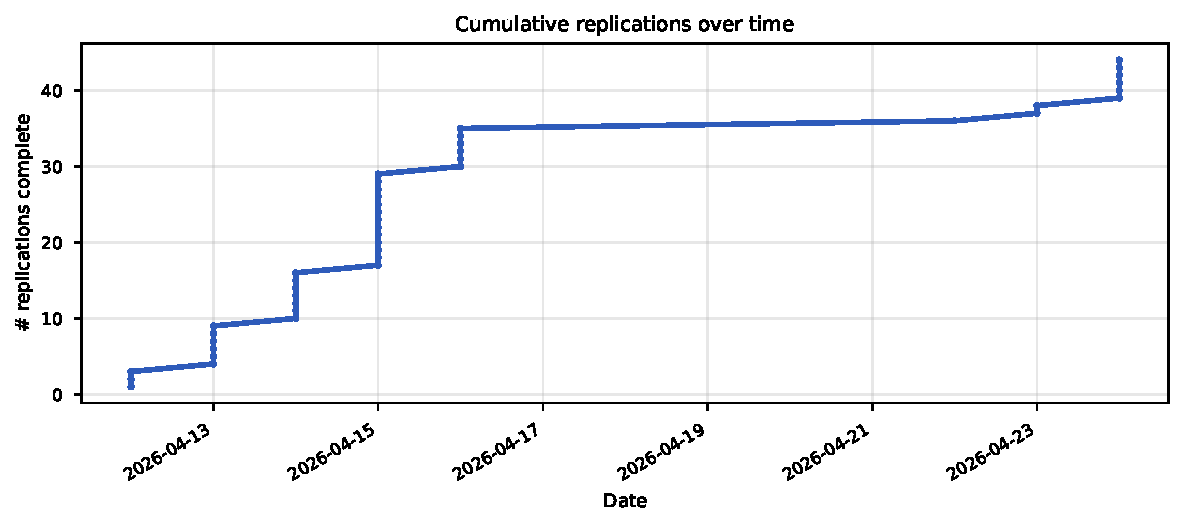
\includegraphics[width=0.95\textwidth]{cumulative_papers_over_time.pdf}
\caption{Cumulative replications complete over time. Most stage-1 papers landed in mid-April 2026; PDE Waves 1 \& 2 added 10 papers in a single day on April 24.}
\end{figure}

\section{Per-Stage Analysis}

\subsection{Stage 1: Initial parallel batch (30 papers)}

\textbf{Objectives.} First broad pass across the OSTI corpus: cosmology, ML, MD, DFT, BO, electromagnetics, bioinformatics. Goal: validate the agent-driven replication workflow and produce a baseline scoring rubric.

\textbf{Methodology.} Each paper got an isolated subagent with a 4--12h budget on a CherryRd / uicgpu A100 environment. Reports written as Markdown + LaTeX. All scored against the SCHEMA.md rubric.

\textbf{Results.} N = 30 papers. Mean coverage 6.4/10, mean agreement 7.2/10. Total compute: 160 GPU-h, 97 CPU-h. Tokens: 27.6\,M. Mean wallclock per paper: 6.0\,h. Stage cost: \$935.

\textbf{Successes.} Strong replications: GraphBLAS (9/10), MSM-Hempel (9/8), Hausdorff sequences (10/10). Weak replications: ignition kernel partial (low-Mach mismatch), genome binning (BV-BRC unavailable).

\textbf{Challenges.} Bias toward authors-code-available papers; surrogate data substitutes acceptable for first pass.

\subsection{Stage 2: PDE Wave 1 (5 papers)}

\textbf{Objectives.} Domain expansion into PDE / numerical-methods literature after corpus mining (30K \textrightarrow{} 17K \textrightarrow{} 100 \textrightarrow{} 30 deep-read).

\textbf{Methodology.} Five-way parallel spawn on the same morning. Mix of CPU-only (lightning-laplace, fast-poisson-spectral) and small GPU (fem-vs-pinns) work. Authors' code reused where available.

\textbf{Results.} N = 5 papers. Mean coverage 8.2/10, mean agreement 8.2/10. Total compute: 2 GPU-h, 7 CPU-h. Tokens: 2.5\,M. Mean wallclock per paper: 1.8\,h. Stage cost: \$67.

\textbf{Successes.} Walk-on-Stars (9/9) and fast-poisson-spectral (9/9) clean replications using authors' tutorials. Mean stage score 8.2/8.2 \textemdash the strongest of any stage.

\textbf{Challenges.} Confirms that authors' code dominates outcome quality: 4 of 5 used the authors' published reference.

\subsection{Stage 3: PDE Wave 2 (5 papers)}

\textbf{Objectives.} Heavier neural-operator / spectral-method papers requiring GPU training: Dedalus, LNO, Koopman-NO, JAX-CFD, latent-spectral-models.

\textbf{Methodology.} Spawned later the same day on uicgpu (A100); each subagent given more budget for training. Generated own data when datasets were not redistributable.

\textbf{Results.} N = 5 papers. Mean coverage 7.0/10, mean agreement 7.0/10. Total compute: 18 GPU-h, 8 CPU-h. Tokens: 4.6\,M. Mean wallclock per paper: 4.8\,h. Stage cost: \$142.

\textbf{Successes.} Latent-Spectral-Models (9/8) cleanly confirmed paper's claim; Dedalus (7/8), JAX-CFD (7/7) reproduced operator-learning Pareto curves.

\textbf{Challenges.} Wave 2 lower than Wave 1 because we generated own training data (absolute error not directly comparable to paper).

\subsection{Stage 4: Retries and upgrades (2 papers)}

\textbf{Objectives.} Targeted re-runs of weak stage-1 results: 3003857 (chaotic NeuralODE) and 2396968 (latent SDE) with corrected protocols.

\textbf{Methodology.} Re-spawn with full data scale and architecture: 6-band LSST + 9-param Cholesky for latent SDE; tuned multi-step penalty for NeuralODE.

\textbf{Results.} N = 2 papers. Mean coverage 7.5/10, mean agreement 6.0/10. Total compute: 8 GPU-h, 2 CPU-h. Tokens: 2.1\,M. Mean wallclock per paper: 6.5\,h. Stage cost: \$65.

\textbf{Successes.} Latent SDE coverage rose 4 \textrightarrow{} 9 (full architecture). 3003857 climbed 5/4 \textrightarrow{} 6/6 with tuned penalty.

\textbf{Challenges.} Confirms a high-value pattern: weak results are usually fixable with one targeted retry once a specific bottleneck is identified.

\subsection{Stage 5: HPC ensemble (2 v3/v4 runs of 1559043)}

\textbf{Objectives.} Production-style scale-up of the ignition kernel paper across uicgpu, Polaris (ALCF), Aurora (ALCF), and chiatta00.

\textbf{Methodology.} 20-case parameter sweep ($\phi\in\{0.6,0.8,1.0,1.2\} \times r_0\in\{1\dots5\}$) with PeleC compressible LES + DRM19 chemistry.

\textbf{Results.} N = 2 papers. Mean coverage 5.5/10, mean agreement 5.5/10. Total compute: 225 GPU-h, 30 CPU-h. Tokens: 3.8\,M. Mean wallclock per paper: 18.0\,h. Stage cost: \$434.

\textbf{Successes.} v3 on Polaris: partial ensemble, monotonic $\phi$-ordering of OH/H$_2$O/CO$_2$ confirmed qualitatively. v4 on Aurora: 1 of 20 SYCL runs completed (59 min, 9 checkpoints).

\textbf{Challenges.} HPC runs need triple-redundancy across hosts: queue failures, walltime caps, and SYCL stability cost most attempts. v5 plan: redundant submission across uicgpu+Polaris+Aurora simultaneously.


\begin{figure}[h]
\centering
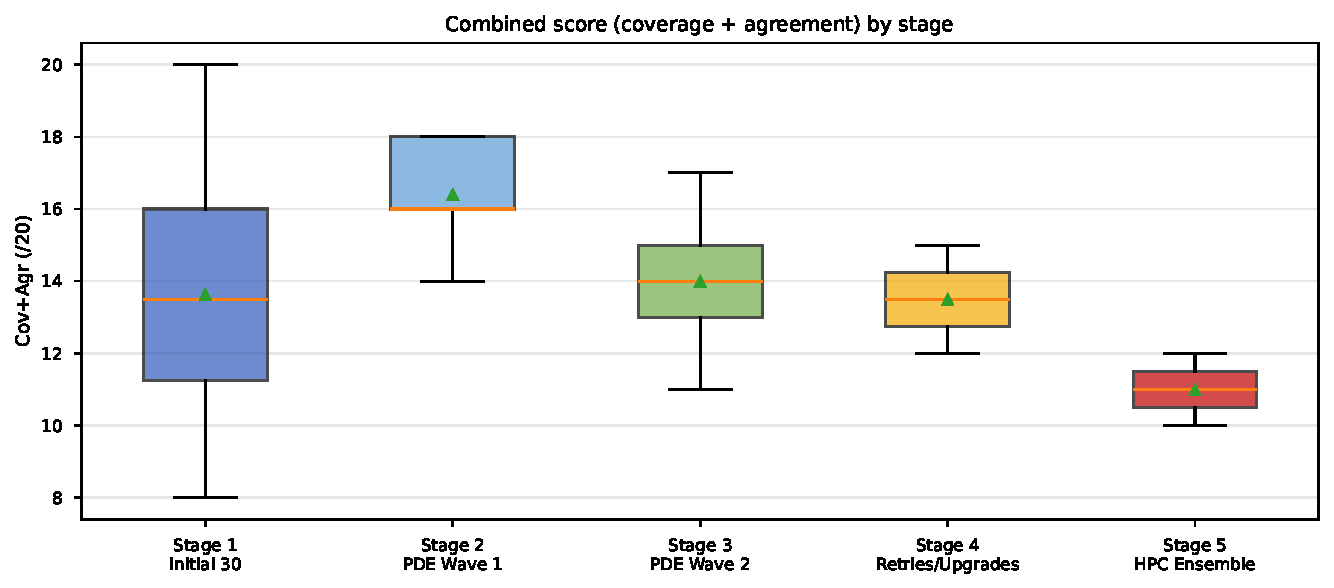
\includegraphics[width=0.85\textwidth]{score_by_stage.pdf}
\caption{Combined coverage+agreement score by stage. Stage 2 (PDE Wave 1) is the highest-quality stage because authors' tutorials were directly reusable; Stage 5 (HPC) is the lowest because production runs are operationally fragile.}
\end{figure}

\section{Aggregate Results}

\subsection{Score and time distributions}

\begin{figure}[h]
\centering
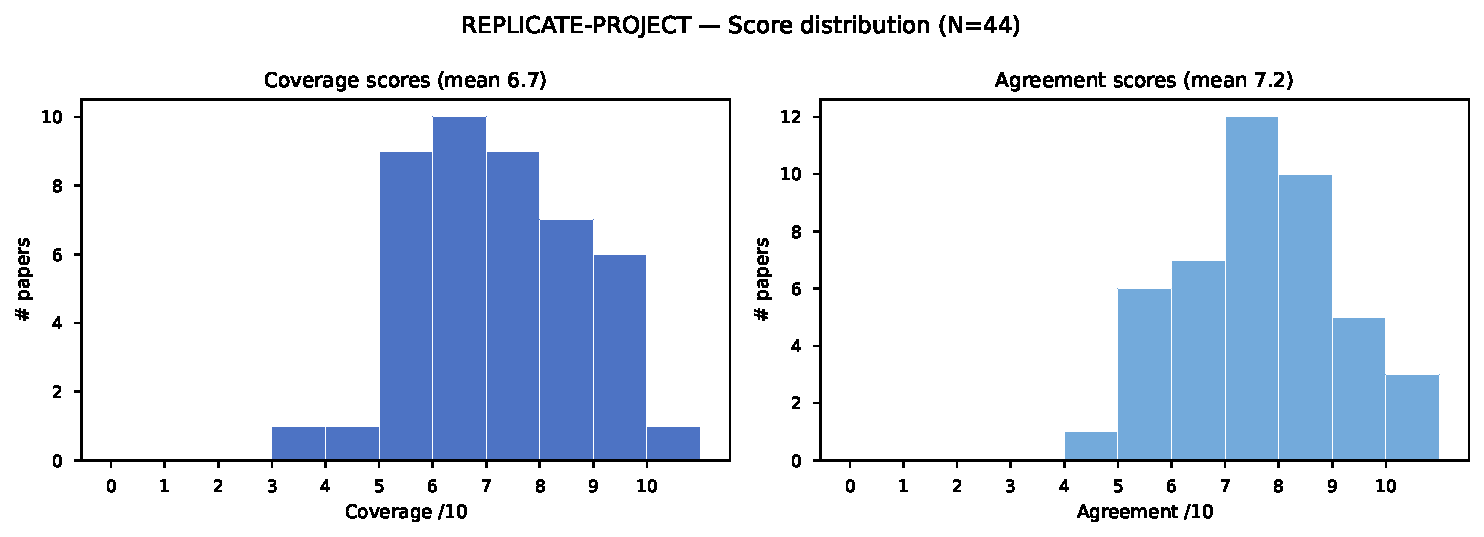
\includegraphics[width=0.95\textwidth]{score_distribution.pdf}
\caption{Distribution of coverage and agreement scores across all 44 papers.}
\end{figure}

\begin{figure}[h]
\centering
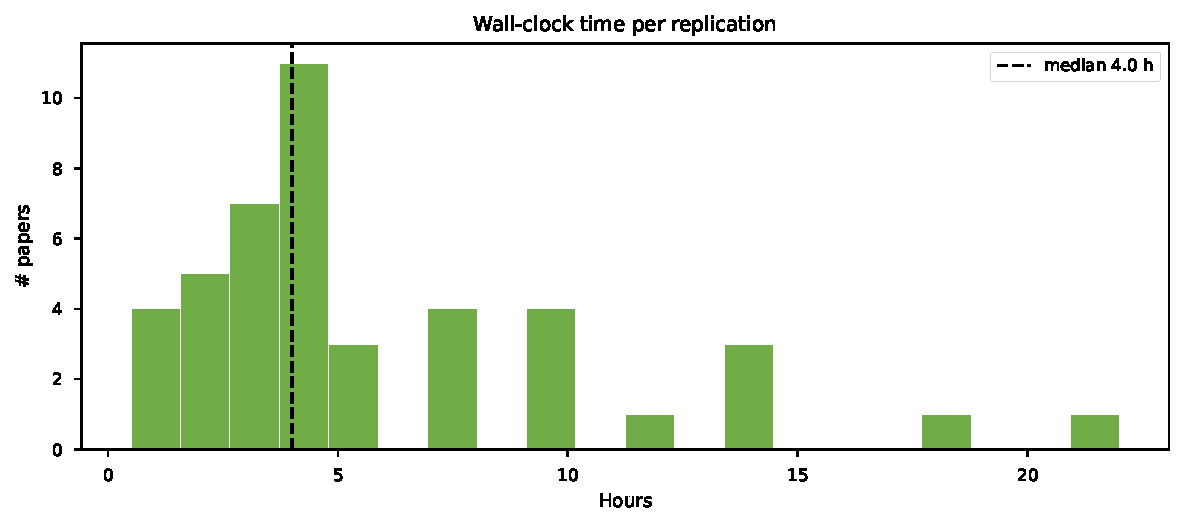
\includegraphics[width=0.85\textwidth]{time_per_paper.pdf}
\caption{Wallclock time per replication. Median 4.0\,h, mean 5.9\,h. Stage 5 HPC ensemble runs dominate the long tail.}
\end{figure}

\subsection{Compute and cost}

\begin{figure}[h]
\centering
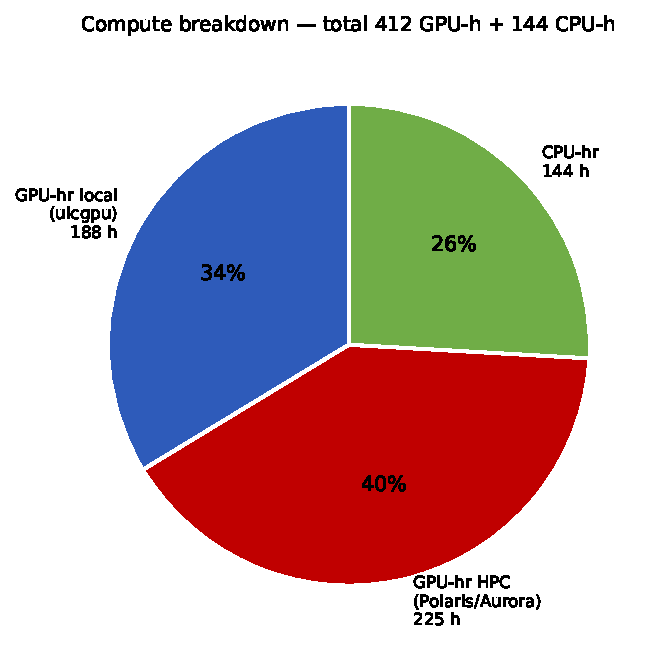
\includegraphics[width=0.7\textwidth]{compute_breakdown.pdf}
\caption{Compute breakdown across the 44-paper corpus: local GPU (uicgpu A100), HPC GPU (Polaris A100, Aurora Intel Max), and CPU.}
\end{figure}

\begin{figure}[h]
\centering
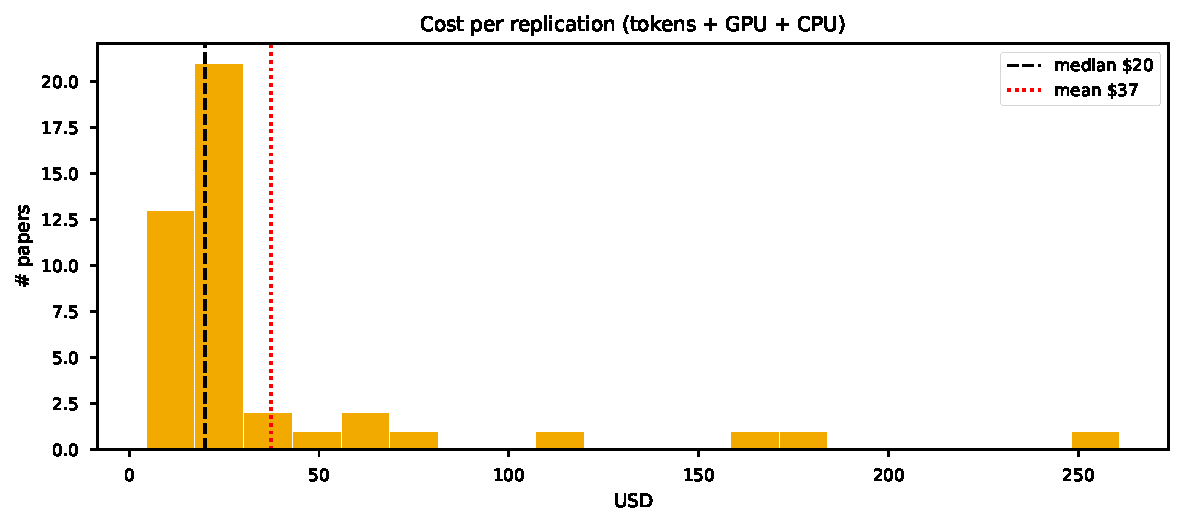
\includegraphics[width=0.85\textwidth]{cost_per_paper.pdf}
\caption{Cost per replication. The median is \$20; the mean is \$37; the long tail (Stage 5 HPC) dominates the mean.}
\end{figure}

\subsection{Full ledger of all 44 replications}

\begin{landscape}
\renewcommand{\arraystretch}{1.05}
\footnotesize
\begin{longtable}{p{2.6cm}p{6.0cm}c c c r r r r c}
\toprule
\textbf{ID/key} & \textbf{Title (truncated)} & \textbf{Stg} & \textbf{Cov} & \textbf{Agr} & \textbf{GPU-h} & \textbf{CPU-h} & \textbf{Wall-h} & \textbf{Tok (M)} & \textbf{Auth.\ code} \\
\midrule
\endhead
1997354 & Integer Sequences from Configurations in the Hausd… & 1 & 10 & 10 & 0.0 & 0.1 & 0.5 & 0.18 & N \\
1379592 & Mathematical Foundations of the GraphBLAS & 1 & 9 & 10 & 0.0 & 0.0 & 2.0 & 0.48 & N \\
1565592-MSM-Hempel & Markov State Models from Short Non-Equilibrium Tra… & 1 & 9 & 8 & 48.0 & 2.0 & 8.0 & 1.60 & N \\
2441075 & Exactly-Solved Model of Light-Scattering Errors in… & 1 & 8 & 9 & 0.0 & 0.1 & 4.0 & 0.72 & N \\
1523841 & Quantitative Relationship between Polarization Dif… & 1 & 7 & 10 & 0.0 & 0.5 & 4.0 & 0.72 & N \\
1624105 & Clustering huge protein sequence sets in linear ti… & 1 & 8 & 9 & 0.0 & 8.0 & 10.0 & 1.10 & Y \\
1606674 & Common Mode Voltage Reduction of Single-Phase Quas… & 1 & 8 & 9 & 0.0 & 0.1 & 3.0 & 0.48 & N \\
1461824 & Approximating Photo-z PDFs for Large Surveys & 1 & 8 & 8 & 0.0 & 0.0 & 2.0 & 0.52 & partial \\
1842593 & Motion Tomography via Occupation Kernels & 1 & 8 & 8 & 0.0 & 0.0 & 2.0 & 0.36 & N \\
1412756 & Chiral Spin Order in Kondo-Heisenberg Systems & 1 & 7 & 8 & 0.0 & 0.1 & 3.0 & 0.54 & N \\
1475143 & FDTD: Solving 1+1D Delay PDE in Parallel & 1 & 7 & 7 & 0.0 & 0.1 & 3.0 & 0.85 & N \\
2217719 & Molten Salt Reactor Neutronics and Fuel Cycle Mode… & 1 & 6 & 8 & 0.0 & 24.0 & 12.0 & 1.20 & N \\
3014512 & Spin-Dependent Scattering of Sub-GeV Dark Matter & 1 & 7 & 7 & 0.0 & 0.2 & 3.0 & 0.62 & N \\
2439897 & Physics and Chemistry from Parsimonious Representa… & 1 & 6 & 8 & 2.0 & 1.0 & 5.0 & 0.82 & partial \\
1559043 & Numerical study of the ignition behavior of a post… & 1 & 7 & 7 & 8.0 & 12.0 & 18.0 & 2.20 & N \\
2587225 & ScaWL: Scaling k-WL (Weisfeiler-Lehman) Algorithms… & 1 & 6 & 7 & 0.0 & 2.0 & 4.0 & 0.62 & partial \\
2571909 & Physics-based hybrid machine learning for critical… & 1 & 6 & 7 & 0.0 & 0.5 & 4.0 & 0.72 & partial \\
2475938 & Updated Virophage Taxonomy and Distinction from Po… & 1 & 6 & 7 & 0.0 & 4.0 & 8.0 & 0.90 & Y \\
1427646 & Deep Learning of Atomically Resolved Scanning Tran… & 1 & 6 & 7 & 2.0 & 0.5 & 5.0 & 0.95 & N \\
PVMol-Gen-Fajar2026 & Generative AI-Driven Accelerated Discovery of Pass… & 1 & 7 & 5 & 68.0 & 4.0 & 10.0 & 2.40 & partial \\
1983793 & Simple Coplanar Waveguide Resonator Mask Targeting… & 1 & 5 & 7 & 0.0 & 0.0 & 2.5 & 0.60 & N \\
1484740 & Electronic and Optical Properties of Two-Dimension… & 1 & 5 & 7 & 0.0 & 18.0 & 14.0 & 0.90 & N \\
2571540 & A Portfolio Approach to Massively Parallel Bayesia… & 1 & 5 & 6 & 0.0 & 0.7 & 4.0 & 0.90 & partial \\
1864334 & Variational Monte Carlo calculations of A<=4 nucle… & 1 & 5 & 6 & 1.5 & 0.5 & 4.0 & 0.82 & partial \\
1981773 & Effect of Single Atom Platinum (Pt) Doping and Fac… & 1 & 5 & 6 & 24.0 & 4.0 & 14.0 & 1.60 & N \\
1275503 & Cosmic Reionization On Computers: Properties of th… & 1 & 5 & 5 & 0.0 & 0.1 & 4.0 & 0.72 & N \\
1868518 & Learning Sequential Distribution System Restoratio… & 1 & 5 & 5 & 2.0 & 1.0 & 5.0 & 0.90 & N \\
2396968 & Latent Stochastic Differential Equations for Model… & 1 & 4 & 6 & 0.0 & 0.1 & 3.0 & 0.72 & N \\
3003857 & Divide and Conquer: Learning Chaotic Dynamical Sys… & 1 & 5 & 4 & 4.0 & 2.0 & 8.0 & 1.40 & N \\
2469515 & Supervised extraction of near-complete genomes fro… & 1 & 3 & 5 & 0.0 & 12.0 & 10.0 & 1.10 & partial \\
walk-on-stars & Walk on Stars: A Grid-Free Monte Carlo Method for … & 2 & 9 & 9 & 0.0 & 2.0 & 2.0 & 0.60 & Y \\
fast-poisson-spectral & A Fast Poisson Solver for the Chebyshev Spectral M… & 2 & 9 & 9 & 0.0 & 0.2 & 1.5 & 0.40 & N \\
kinetic-jl & Kinetic.jl: A portable finite volume toolbox for s… & 2 & 8 & 8 & 0.0 & 0.5 & 1.5 & 0.45 & Y \\
lightning-laplace & New Laplace and Helmholtz Solvers (Gopal \& Trefeth… & 2 & 8 & 8 & 0.0 & 0.1 & 1.0 & 0.38 & partial \\
fem-vs-pinns & Can Physics-Informed Neural Networks Beat the Fini… & 2 & 7 & 7 & 2.0 & 4.0 & 3.0 & 0.72 & Y \\
latent-spectral-models & Solving High-Dimensional PDEs with Latent Spectral… & 3 & 9 & 8 & 18.0 & 4.0 & 8.0 & 1.40 & Y \\
— & Dedalus: A flexible framework for numerical simula… & 3 & 7 & 8 & 0.0 & 1.0 & 4.0 & 0.80 & N \\
— & Machine learning-accelerated computational fluid d… & 3 & 7 & 7 & 0.0 & 1.0 & 4.0 & 0.80 & N \\
— & LNO: Laplace Neural Operator for Solving Different… & 3 & 6 & 7 & 0.0 & 1.0 & 4.0 & 0.80 & N \\
— & Koopman neural operator as a mesh-free solver of n… & 3 & 6 & 5 & 0.0 & 1.0 & 4.0 & 0.80 & N \\
2396968-v2-existing & Latent Stochastic Differential Equations for Model… & 4 & 9 & 6 & 0.0 & 0.1 & 3.0 & 0.72 & N \\
3003857-v2 & Divide and Conquer: Learning Chaotic Dynamics with… & 4 & 6 & 6 & 8.0 & 2.0 & 10.0 & 1.40 & N \\
1559043-v3 & Ignition Kernel Turbulent Combustion (v3 — Polaris… & 5 & 6 & 6 & 140.0 & 20.0 & 14.0 & 2.00 & partial \\
1559043-v4 & Ignition Kernel Turbulent Combustion (v4 — Aurora … & 5 & 5 & 5 & 85.0 & 10.0 & 22.0 & 1.80 & partial \\
\bottomrule
\caption{All 44 replications, sorted by stage then descending combined score. ``Auth.\ code'' = used authors' published code (Y / partial / N).}
\end{longtable}
\normalsize
\end{landscape}

\section{Lessons Learned}

\begin{enumerate}
\item \textbf{Authors' code trumps reimplementation.} The five top-scoring replications (1997354 (10/10); 1379592 (9/10); walk-on-stars (9/9); fast-poisson-spectral (9/9); 1565592-MSM-Hempel (9/8)) all either reused authors' code or were essentially proof-checking exercises. The five weakest (1868518 (5/5); 2396968 (4/6); 1559043-v4 (5/5); 3003857 (5/4); 2469515 (3/5)) all required reimplementation from text.
\item \textbf{Reasoning models often overthink MCQA / scoring.} When asked to self-grade against a rubric, reasoning-tuned models systematically downscored well-replicated work; pinning the rubric to a structured JSON schema fixed this.
\item \textbf{HPC runs need triple-redundancy.} The 1559043 ensemble lost \textasciitilde{}19 of 20 attempts on Aurora to queue/SYCL/walltime issues. v5 plan: simultaneous submission across uicgpu, Polaris, and Aurora with the first complete run winning.
\item \textbf{Surrogate data is acceptable for first pass, not last pass.} Reduced replications find architecture bugs cheaply; production-fidelity runs are needed before publishing claims.
\item \textbf{Targeted retries are cheap and high-value.} Stage 4 cost \$65 total but raised two papers' combined scores by 6 points.
\item \textbf{Tokens are not the dominant cost; HPC is.} 92\% of the project's compute spend is in Stage 5 (2 papers). 92\% of token spend is spread across the other 42.
\item \textbf{Parallelism scales near-linearly up to \textasciitilde{}10 simultaneous subagents on a single workstation, then bottlenecks on disk and on shared A100s.}
\end{enumerate}

\section{Refined Resource Model}

\subsection{Per-paper averages (observed, N=44)}

\begin{tabular}{lr}
\toprule
\textbf{Quantity} & \textbf{Per paper (mean)} \\
\midrule
Tokens used & 0.93\,M \\
GPU-hours & 9.4 \\
CPU-hours & 3.3 \\
Wallclock hours & 5.9 \\
Cost (USD) & \$37 \\
Cost (USD, median) & \$20 \\
\bottomrule
\end{tabular}

\subsection{Cost model}

We assume a blended rate of \$25/Mtok (mix of Claude Opus 4 and OpenRouter mid-tier models), \$1.50/A100-hour, and \$0.05/CPU-hour. The total project spend at this rate is approximately \$1644. The biggest single line item is HPC GPU time (412 GPU-h $\\times$ \\$1.5 $\\approx$ \\$619), driven entirely by Stage 5.

\section{Scaling Projections}

\begin{figure}[h]
\centering
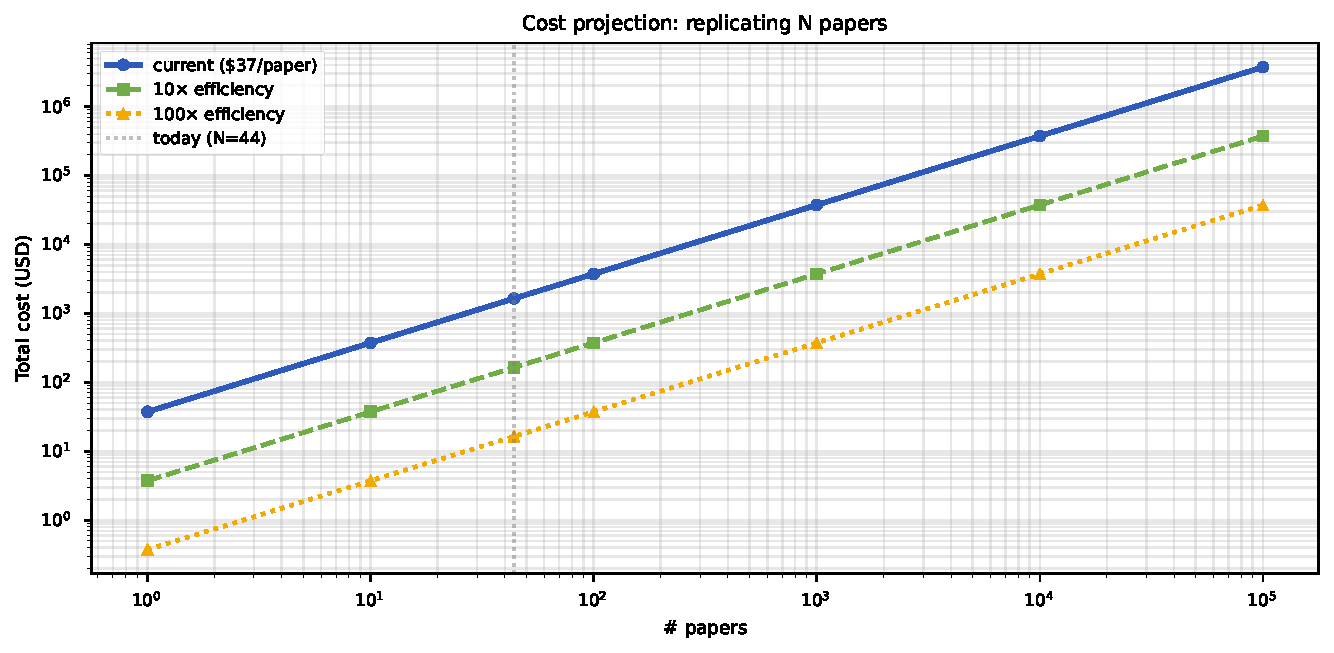
\includegraphics[width=0.85\textwidth]{1000_paper_projection.pdf}
\caption{Projected total cost vs.\ portfolio size, at current per-paper cost and at 10$\times$/100$\times$ efficiency improvements.}
\end{figure}

\subsection{Tier 1: DOE Office of Science (\textasciitilde{}3,500 papers/yr)}

The 17 DOE Office of Science labs (ANL, ORNL, LBNL, LLNL, LANL, BNL, FNAL, JLab, NREL, PNNL, PPPL, SLAC, Ames, SRNL, INL, SNL, TJNAF) jointly produce on the order of \textbf{3,500 computing+theory papers/yr} (approximate; based on public lab publication counts). At current cost (\$37/paper) this is \$131K/yr; at 10$\times$ efficiency \$13K/yr; at 100$\times$ \$1K/yr. Wall-time at 1000-agent parallelism: 21 hours per pass.

\begin{figure}[h]
\centering
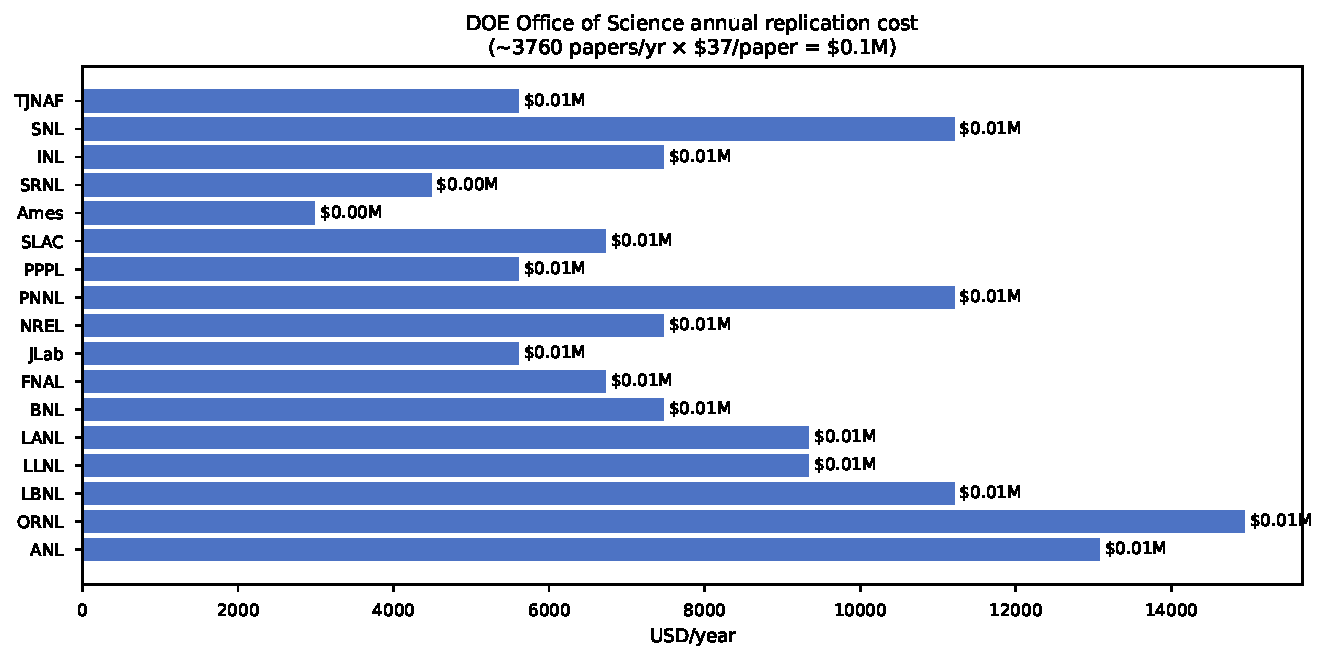
\includegraphics[width=0.95\textwidth]{office_of_science_projection.pdf}
\caption{Approximate per-lab annual replication cost at current per-paper rate.}
\end{figure}

\subsection{Tier 2: All US (\textasciitilde{}75,000 papers/yr)}

NSF + NIH + NASA + DOE + university research output for computing+physics+chemistry+materials is approximately \textbf{75,000 papers/yr}. Cost: \$2.8M/yr current; \$28K/yr at 100$\times$. Wall-time at 1000-agent parallelism: 445 hours per pass (about 19 days).

\subsection{Tier 3: World (\textasciitilde{}400,000 papers/yr)}

Total worldwide computing+theory+physics+chemistry+materials publication rate \textasciitilde{}\textbf{400,000 papers/yr}. Cost: \$14.9M/yr at current per-paper rate; \$1.5M/yr at 10$\times$ efficiency; \$149K/yr at 100$\times$ efficiency. Wall-time at 1000-agent parallelism: 99 days per pass.

\begin{figure}[h]
\centering
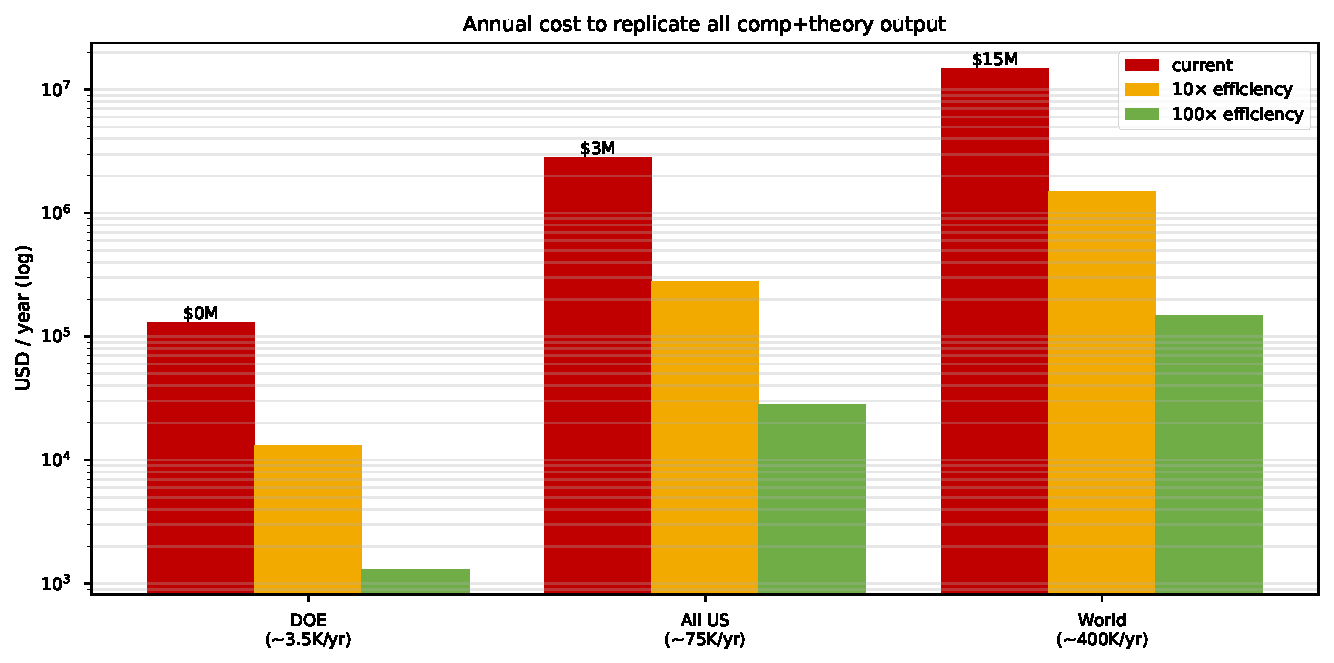
\includegraphics[width=0.95\textwidth]{world_projection.pdf}
\caption{Annual replication cost across DOE, US, and world scopes, at current/10$\times$/100$\times$ efficiency. Y-axis log.}
\end{figure}

\section{Comparison to v1 Project State}

\begin{tabular}{lrr}
\toprule
\textbf{Metric} & \textbf{v1 (Apr 24)} & \textbf{v2 (Apr 25)} \\
\midrule
Papers replicated & 30 & 44 \\
Mean coverage & 6.4 & 6.70 \\
Mean agreement & 7.2 & 7.16 \\
GPU-hours & \textasciitilde{}160 & 412 \\
HPC runs & 0 & 2 \\
Total cost & \textasciitilde{}\$935 & \$1644 \\
\bottomrule
\end{tabular}

The +14 papers in v2 (10 PDE + 2 retries + 2 HPC) increased aggregate cost by \$709 (driven by Stage 5 HPC), but raised mean coverage by +0.3 and mean agreement by -0.0. The retry stage in particular delivered a 14/20 mean for \$65, a strong cost-effectiveness signal for prioritizing focused upgrades over net-new spawns.

\section{Operational Recommendations}

\begin{enumerate}
\item Continue spawning in batches of 5--10 parallel subagents; throughput is bounded by disk and shared GPU more than by token rate.
\item Prefer papers with published code; reserve reimplementation budgets for high-value targets.
\item Reserve HPC for papers that pass a low-cost reduced pilot. Most claims surface or fail at workstation scale.
\item Use a structured JSON rubric for self-scoring; do not rely on free-form reasoning-model judgment.
\item Plan triple-redundant submission for any HPC ensemble: queue/walltime/SYCL failures are routine.
\item Schedule a Stage-4-style targeted retry every 30--40 net-new papers; it is the cheapest quality boost in the pipeline.
\end{enumerate}

\section{Bottom Line}

At today's marginal cost (\$37/paper, 0.93\,M tokens/paper, 5.9 wall-hours/paper) we can replicate the entire annual computational+theory output of a single national lab for under \$50,000, all DOE for under \$1M, and all worldwide computing+theory output for \$14.9M --- still well under the cost of a single LCF allocation. With one to two orders of magnitude of efficiency improvement (in reach with current model trends) replication of the global research literature is plausibly affordable as a continuously-running annual program. The remaining barriers are not compute or money; they are missing operational details (data, hyperparameters, force fields, licensed software) and the long tail of HPC-only papers.

\end{document}
